\subsection{Diffuse Supernova Neutrino Background - M Wurm, J Sawatzki}

%\paragraph{Motivation}

The Diffuse Supernova Neutrino Background (DSNB) consists of neutrinos emitted by all core-collapse Supernovae (SNe) throughout the Universe. Red-shifted by cosmic expansion and travelling over vast distances, these neutrinos constitute a faint isotropic background flux. The discovery and subsequent spectroscopy of the DSNB will provide unique information on the redshift-dependent SN rate, the relative frequency of neutron star and black hole formation and the EoS of the emerging neutron stars.

The primary detection reaction is the Inverse Beta Decays (IBD) induced by the $\bar\nu_e$ component of the DSNB. With an expected event rate of 0.1 per year and kiloton of detector material, overwhelming backgrounds have to be faced. However, with SK-Gd and JUNO there are now two contenders with a realistic chance to obtain a first ($3\sigma$) evidence of the DSNB within the next 5-10 years.

%Still, within the likely observation window between 10 and 30\,MeV the faint signal is within reach of current and upcoming large-volume neutrino detectors.

%The best limit of 2.9\,cm$^{-2}$s$^{-1}$ (integral $\bar\nu_e$ flux for $E_\nu>17.3$\,MeV)  on the DSNB flux has been obtained by the Super-Kamiokande experiment \cite{Bays:2011si}. Its recent upgrade to a gadolinium-loaded water target (SK-Gd) will greatly enhance its sensitivity, likely to provide it with a first glance of the DSNB. However, the rather limited event rate of 2-3 events per year means that a first evidence of the signal is still many years away. A similar argument can be made for the liquid-scintillator detector JUNO. Coming online in 2021, it will have to collect data for many years to reach a $3\sigma$ significance level \cite{}.

THEIA may play a pivotal role in the discovery and exploration of the DSNB signal. Based on a target mass twice the size of SK or JUNO, it will accumulate statistics much faster. Moreover, the dual detection of Cherenkov and scintillation signal offers a background discrimination capability unparalleled by Gd-doped water or pure organic scintillator, resulting in an expected signal efficiency close to unity ($\sim$97\,\%) within the observation window. 

\subsubsection{DSNB signal and background levels}

For IBD events, the prompt energy of the positron signal translates almost directly to the incident neutrino energy, while the delayed neutron capture provides a fast coincidence tag to reduce the ample single-event backgrounds. Figure \ref{fig:dsnb_spectrum}a) depicts the visible energy spectrum (scintillation only) for the prompt positrons. The chosen detector configuration corresponds to a WbLS of 10\,\% organic fraction and 70\,\% photocoverage, resulting in a photoelectron yield of 120 (80) for scintillation (Cherenkov) component. The DSNB model is based on work by the Garching group \cite{}. 

Figure \ref{fig:dsnb_spectrum}a) shows as well the relevant background spectra: IBDs from {\it reactor and atmospheric} $\bar\nu_e$'s constitute an indistinguishable background that overwhelms the signal at low and high energies, effectively limiting the detection to an energy window of 10--30\,MeV. 

%The flux normalization translates to 0.29 events per kiloton$\cdot$year.

%Excited nuclei and nuclear fragments created by the NC interactions of atmospheric neutrinos can be efficiently discriminated by the Cherenkov/Scintillation (C/S) ratio, allowing for a low-background DSNB event sample at very high detection efficiency. Measuring background levels precisely in a similar target medium, THEIA will as well help reduce the systematic uncertainties of the SK-Gd and JUNO measurements.

%In both cases, the main challenge: very low signal rate in the presence of considerable backgrounds
%n water and LS, primary detection channel is the inverse beta decay; neutron tagging capability vastly improves the chances for a positive detection
%still, on a level fo only 1 event per 10 kt-yrs, even minor background rates become a formidable challenge
%a convincing discovery therefore must provide both sufficient event statistics and a clear signature for separating DSNB and background events based on the prompt signal


%Given the multitude and distance of Supernovae (SNe) contributing to the overall background flux, the DSNB signal results from a nearly isotropic neutrino flux with a  spectrum averaged for all types of core-collapse SN, substantially red-shifted for Supernovae at far-out distances. The detectable signal above 10 MeV (see below) is thus dominated by SNe out to red-shifts of $z\approx1$. 

%For IBD events, the prompt energy of the positron signal translates almost directly to the incident neutrino energy, while the delayed neutron signal provides a fast coincidence tag to reduce the ample single-event backgrounds. Figure \ref{fig:dsnb_spectrum} depicts the visible energy spectrum (scintillation only) for the prompt positrons. The underlying SN model and $z$-dependent Supernova rate we used the reference model of the Garching group \cite{}. The used detector configuration is close to {\it THEIA-ii}: Energy scale and resolution correspond to a photoelectron yield of 120 per MeV of deposited energy, corresponding to 10\,\% organic ratio in the WbLS and a photocoverage of 70\,\%. The flux normalization translates to 0.29 events per kiloton$\cdot$year.

\begin{figure}[b!]
\centering
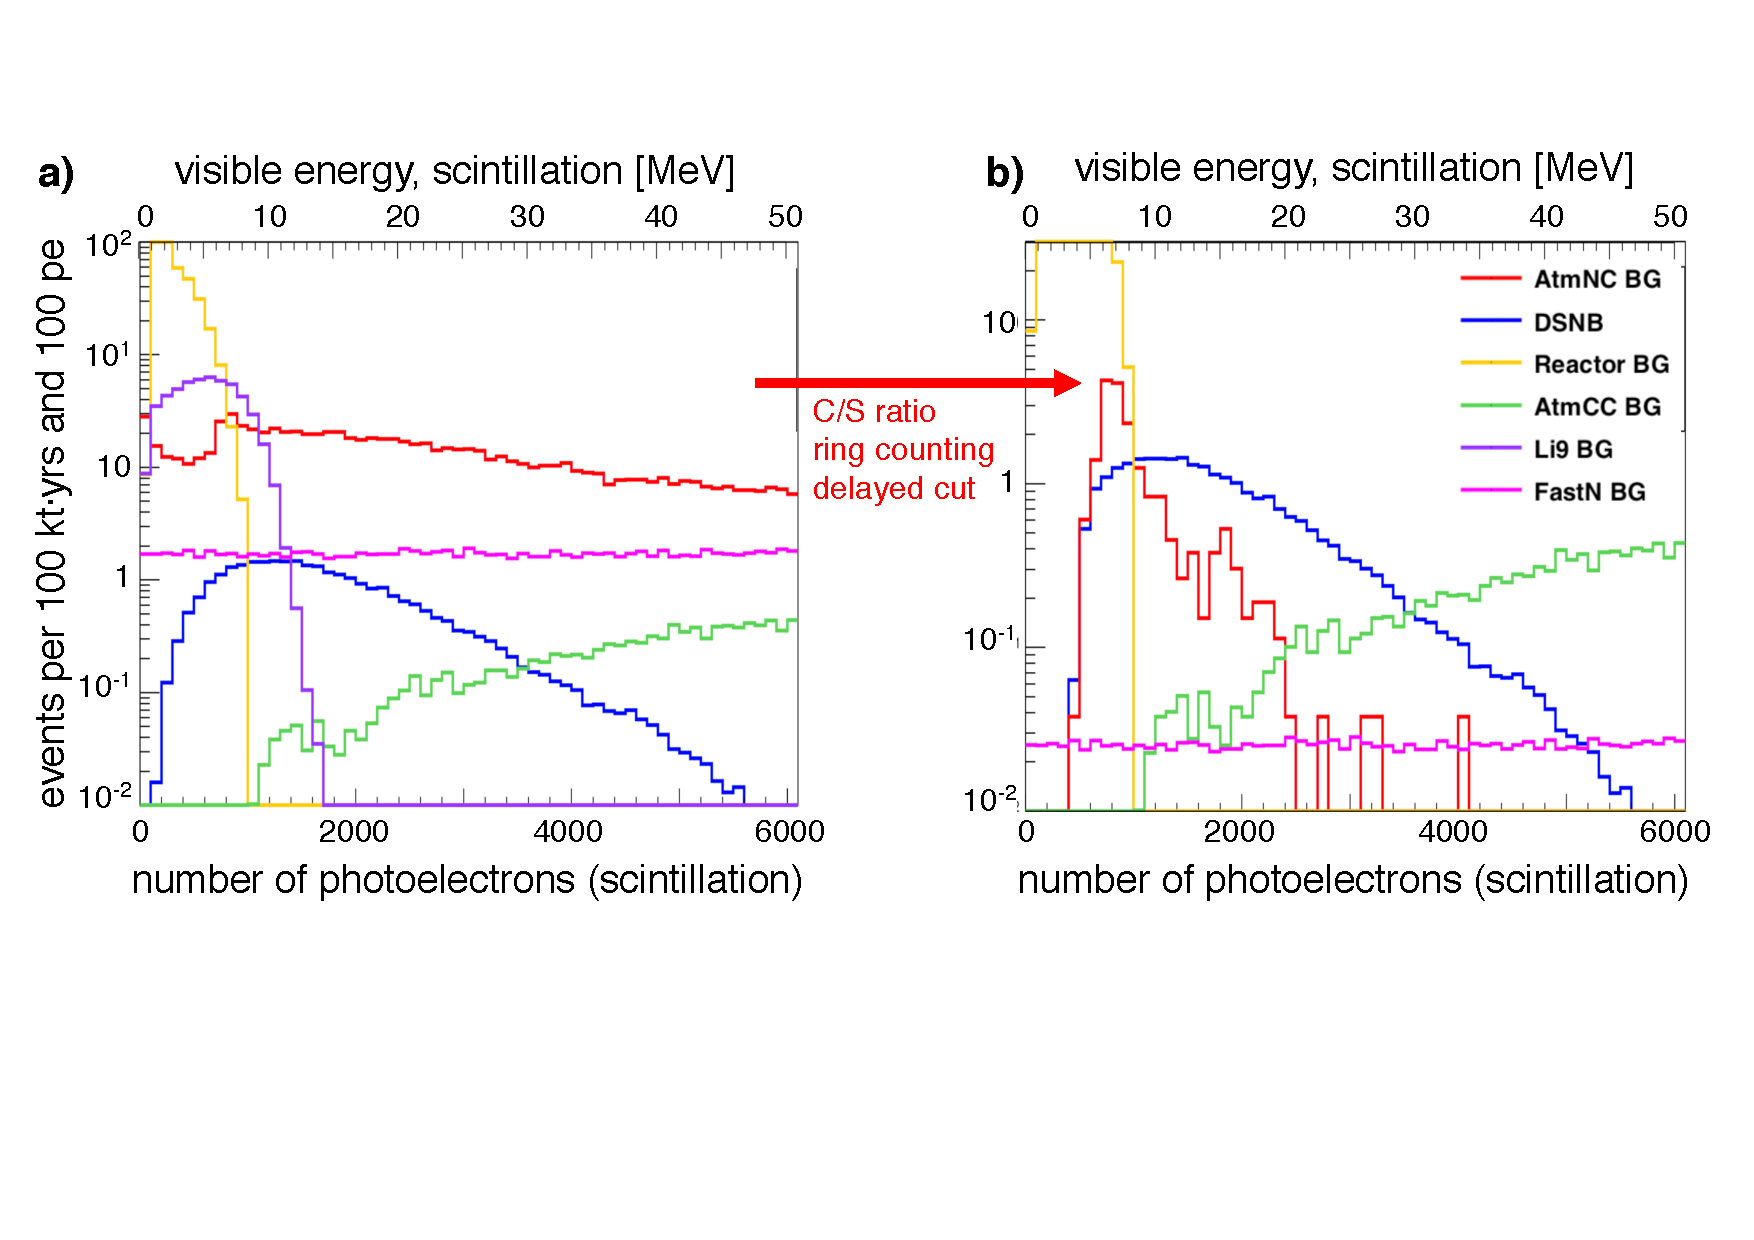
\includegraphics[width=0.9\textwidth]{pics/dsnb_spectrum_theia}
\caption{The visible scintillation energy spectrum expected for the DSNB signal and its ample backgrounds. The presented spectra include reactor neutrinos, cosmogenic Li-9, fast neutrons as well as atmospheric neutrino CC and NC interaction rates before application of discrimination techniques. The irreducible antineutrino backgrounds limit the observation window to the range of $\sim$8 to 30\,MeV.}
\label{fig:dsnb_spectrum}
\end{figure}

%As indicated in figure \ref{fig:dsnb_spectrum}, the faint DSNB signal is beset by a variety of backgrounds. The observation window is set by two irreducible $\bar\nu_e$ backgrounds that themselves induce IBDs: {\bf Reactor neutrinos} constitute an overwhelming background for terrestrial detectors and limit the detection in the energy range below $\sim$8 MeV. At higher energies, {\bf CC interactions of atmospheric neutrinos} start to dominate the DNSB rate from $\sim$30\,MeV. These two backgrounds define the observation window for all water and LS detectors.

But even within this window, several further background sources contribute, all of cosmogenic origin: {\it cosmogenic $\beta n$-emitters}, primarily $^9$Li, are created by muon spallation on the oxygen (and carbon) nuclei of the target; {\it fast neutrons} are induced by muons in the rock surrounding the detector and are able to enter the detector unnoticed. The combination of a prompt signal created by elastic scattering off protons and the subsequent neutron capture may mimic the IBD signature. Finally,  {\it NC reactions of atmospheric neutrinos (atm-NC)} resemble the IBD coincidence in case a prompt signal is generated due to the recoils and possible de-excitation of the fragments of the target nucleus and a delayed signal in case a neutron is released from the nuclear break-up. First recognized by the KamLAND experiment for its special importance in organic scintillators, it dominates the DSNB signal by more than one order of magnitude. For scintillator detectors like JUNO, the quenched nuclear signal constitutes a major challenge to be overcome by pulse shape discrimination. SK-Gd will be much less affected but features this background as well below $\sim$16\,MeV.

%Finally,   constitute the most serious background to DSNB detection.  The IBD-mimicking events originate from reactions with a single neutron in the final state, while the prompt signal can be composed from a multitude of different combinations of nuclear fragments and gamma-rays.  

%The only isotope produced at a relevant cross-section and providing a $\beta$-signal of sufficiently high energy to reach into the observation window is $^9$Li. Depending on the depth of the detector, this background can be efficiently suppressed by forming a time-coincidence veto with the parent muon. 
%\item {\bf Fast neutrons} are induced by muons passing the rock surrounding the detector and can in principle enter the detector unnoticed. The combination of a prompt signal created by elastic scattering off protons and the subsequent neutron capture can mimic the IBD signature. Since these events enter the detector from outside, they can be effectively addressed by a fiducial volume cut. Moreover, a cut on the C/S ratio will as well reduce this background contribution.
%\item {\bf NC reactions of atmospheric neutrinos} constitute the most serious background to DSNB detection.  The IBD-mimicking events originate from reactions with a single neutron in the final state, while the prompt signal can be composed from a multitude of different combinations of nuclear fragments and gamma-rays.  First recognized by the KamLAND experiment for its special importance in organic scintillators, it dominates the DSNB signal by more than one order of magnitude. For detectors featuring delayed neutron-tagging capabilities (like JUNO and to some extent as well SK-Gd), discrimination of this background is the major challenge.
%\end{itemize}

\subsubsection{Background discrimination in WbLS} 

The major virtue of THEIA lies with its excellent background discrimination capabilities: In context of the DSNB search, the following have been investigated:

\begin{itemize}
\item {\it Distance cuts} relative to passing muons to veto $^9$Li-days and defining an inner fiducial volume to reject fast neutrons reduce these backgrounds to a negligible level.
\item {\it Delayed decays:} In almost 50\,\% of the relevant atm-NC events, the residual nucleus is the $\beta^+$-emitting isotope $^{15}$O that undergoes a taggable $\beta^+$-decay with a lifetime of 2.2\,min.

%The dominant NC reaction partner of atmospheric neutrinos in WbLS are oxygen nuclei. This turns out to be an advantage over organic LS where interactions on carbon predominantly create the long-lived isotope C-11. Contrariwise, the most ample isotope created in WbLS is O-15. It's subsequent $\beta$-decay with an endpoint of 2.5\,MeV and lifetime of 2.2\,min will be well visible in a WbLS detector and allows to remove about half of the NC background events by searching for a three-fold coincidence of prompt, delayed and a late O-15 decay event (see table \ref{fig:dsnb_delayed_tagging} for the relevant branching ratio). While a similar argument can be made for the low-yield B-12, all other isotopes are either stable or decaying too fast for a delayed tag.
%\begin{figure}[htp!]
%\centering
%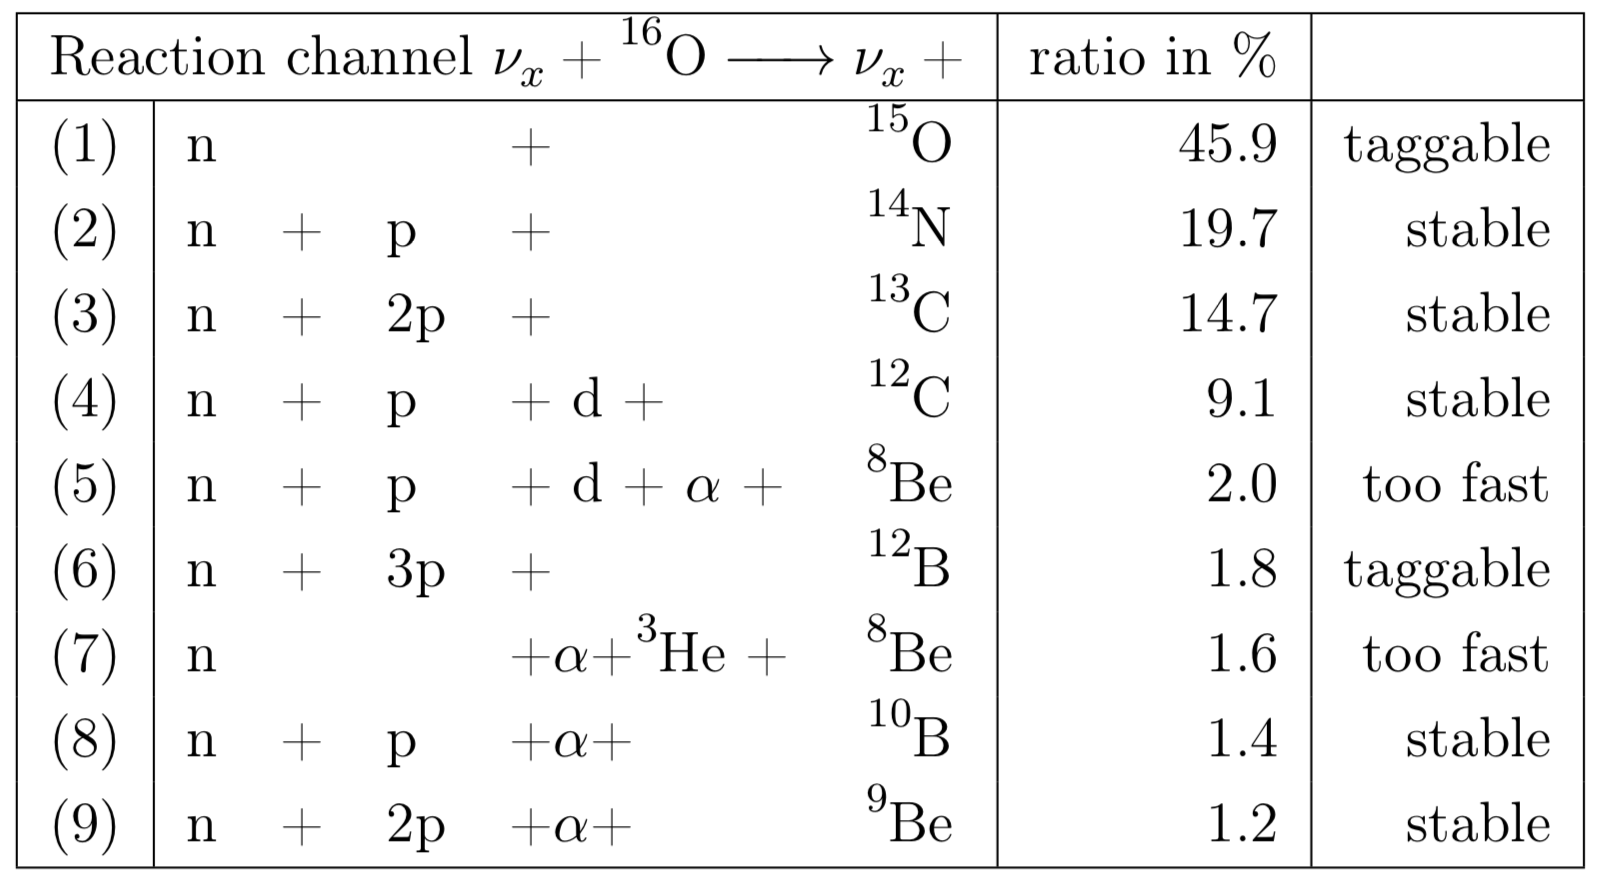
\includegraphics[width=0.55\textwidth]{dsnb/dsnb_delayed_tagging}
%\caption{Inelastic NC reactions of atmospheric neutrinos on O-16 often remove n%ucleons so that a fragmented nucleus remains in the final state. In the case of O-15 and B-12, the residual nuclei are unstable, allowing the identification of the NC background by a threefold-coincidence tag including the delayed radioactive decay of the isotope.}
%\label{fig:dsnb_delayed_tagging}
%\end{figure}
\item {\it C/S ratio:} The main virtue of WbLS detectors is the possibility to discriminate events by the magnitude  of the Cherenkov signal accompanying the scintillation light. While $e^\pm$ and $\gamma$ signals feature a high C/S ratio, that of non-relativistic nuclear recoils practically zero. As demonstrated by the left panel of Fig.~\ref{fig:dsnb_csratio} that displays the C/S ratios of signal and atm-NC events as a function of visible energy, this parameter provides a powerful tool to reject atm-NC (but also fast neutron) background events. Perfect separation is inhibited by a curved band of atm-BG events featuring non-zero C/S values due to $\gamma$-production by nuclear de-excitations of the final state. The right panel of Fig.~\ref{fig:dsnb_csratio} describes the relation between DSNB signal efficiency and atm-BG residual fraction that can be achieved by a cut on the C/S ratio. In the following, we adapt 98\,\% signal efficiency and 5\,\% background acceptance.

%a cut on the C/S ratio of the photon signal, allowing to discriminate different particle types by their Cherenkov light emission (or its absence). In the present case, positron-like IBDs can be separated from the mixed and largely hadronic prompt events in both atmospheric NC and fast neutron interactions. The left panel of figure~\ref{fig:dsnb_csratio} demonstrates the discrimination power by plotting the C/S ratio of DSNB signal and atmospheric NC background as function of the visible scintillation energy: For visible energies greater than 8\,MeV (1,000\,p.e.), the distributions of both species are clearly separated.

%The residual background contamination arises from NC reactions in which gamma-rays are produced as a side-product: they may either originate from nuclear excitations directly induced by the reaction ($E_\gamma\leq20$\,MeV) or are often released in secondary neutron interactions with O-16, featuring a typical energy of $\sim$6\,MeV. The latter create an easy-to-spot curved band in the distribution of atmospheric NC events in figure~\ref{fig:dsnb_csratio}. Due to these events, the discrimination is not perfect but nevertheless provides a potent pool to reduce the spectral contribution of atmospheric NC neutrinos. A corresponding curve evaluating the residual of atmospheric NC events as a function of positron acceptance is depicted in figure~\ref{fig:dsnb_csratio}: For instance, NC backgrounds can be reduced by 95\,\% while maintaining a DSNB signal acceptance of 98\,\%.

\item {\it Ring counting:} The reconstruction of Cherenkov rings from individual final-state particles provides a further handle to discriminate one-ring positron events from multi-ring atm-NC events. From simulation, we find that about 60\,\% of the latter background events can be discriminated based on this feature\footnote{For this, we require that the subleading ring features at least 20\,\% of the overall Cherenkov photons.}, introducing a negligible loss in signal efficiency.


% Figure~\ref{fig:dsnb_multiring_disc} shows the number of Cherenkov rings in NC events as a function of the visible scintillation energy. By limiting the signal acceptance to one-ring events, about 2/3 of the background events can be discriminated without any relevant signal loss. If we assume that the second Cherenkov ring must contain at least 20\,\% of the photons to be discernible from the dominant one, the expected background rejection efficiency is still 60\,\%.
%\begin{figure}[htp!]
%\centering
%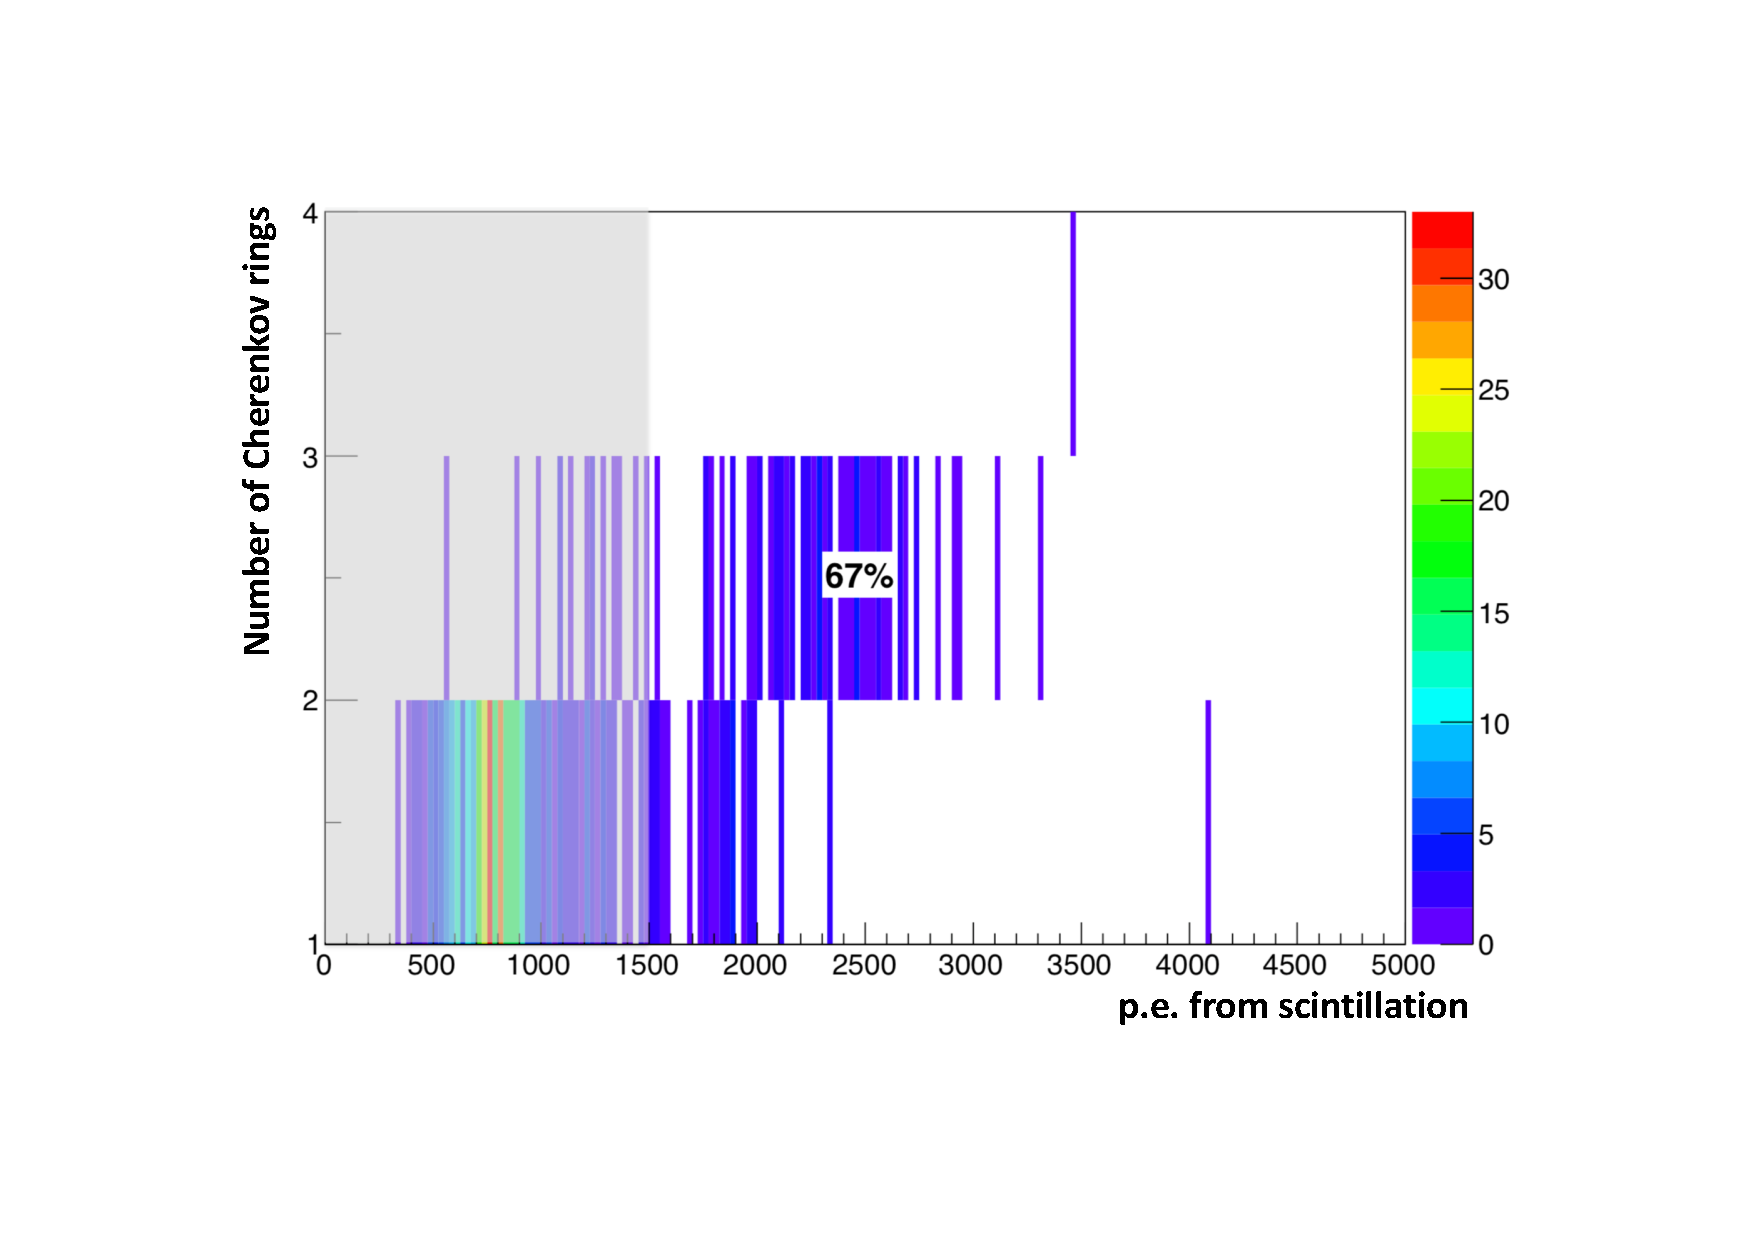
\includegraphics[width=0.55\textwidth]{dsnb/dsnb_multiring_disc}
%\caption{Number of Cherenkov rings reconstructed for atmospheric NC events as a function of the prompt visible scintillation energy. The frequent occurrence of two or more rings allows for an efficient discrimination against the single-ring DSNB positrons.}
%\label{fig:dsnb_multiring_disc}
%\end{figure}

\end{itemize}

\begin{figure}[htp!]
\centering
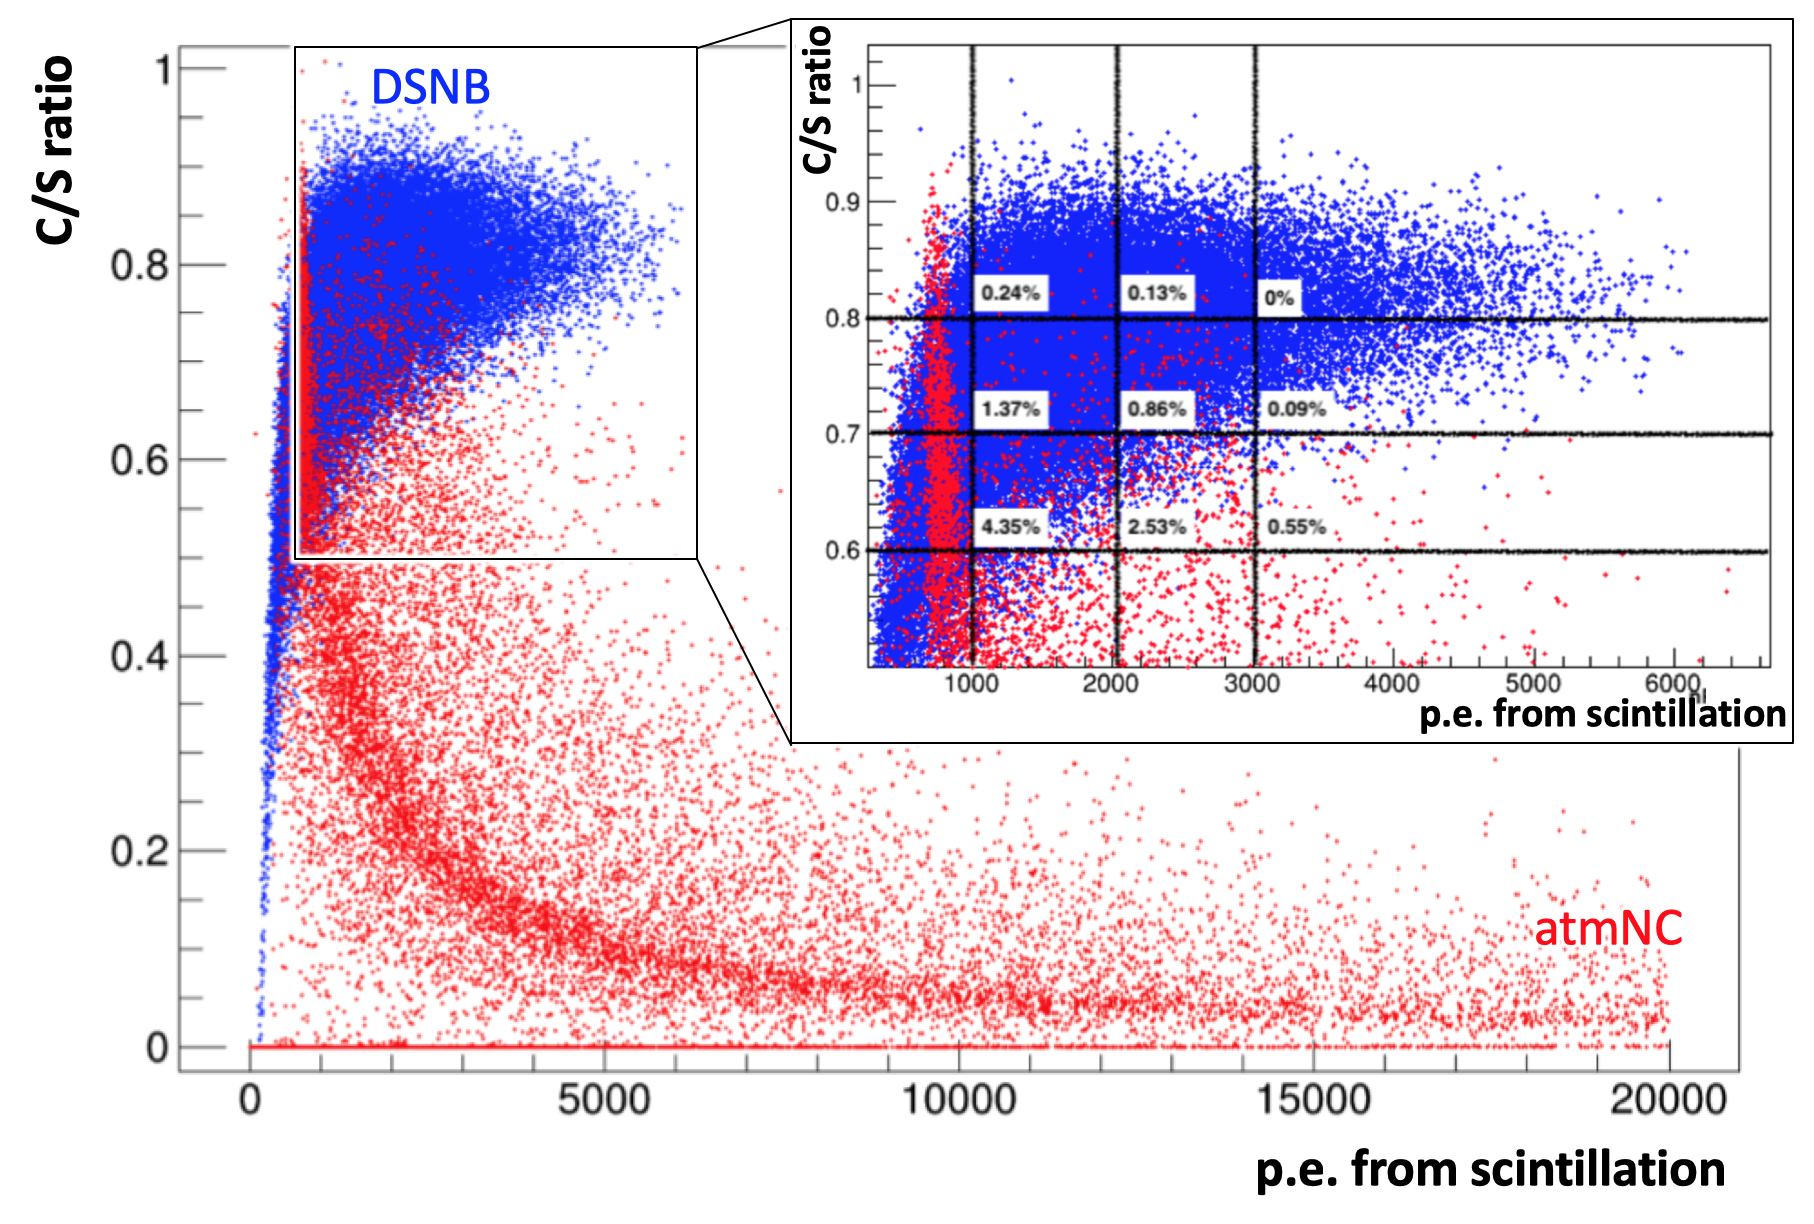
\includegraphics[width=0.6\textwidth]{pics/dsnb_cs_ratio}
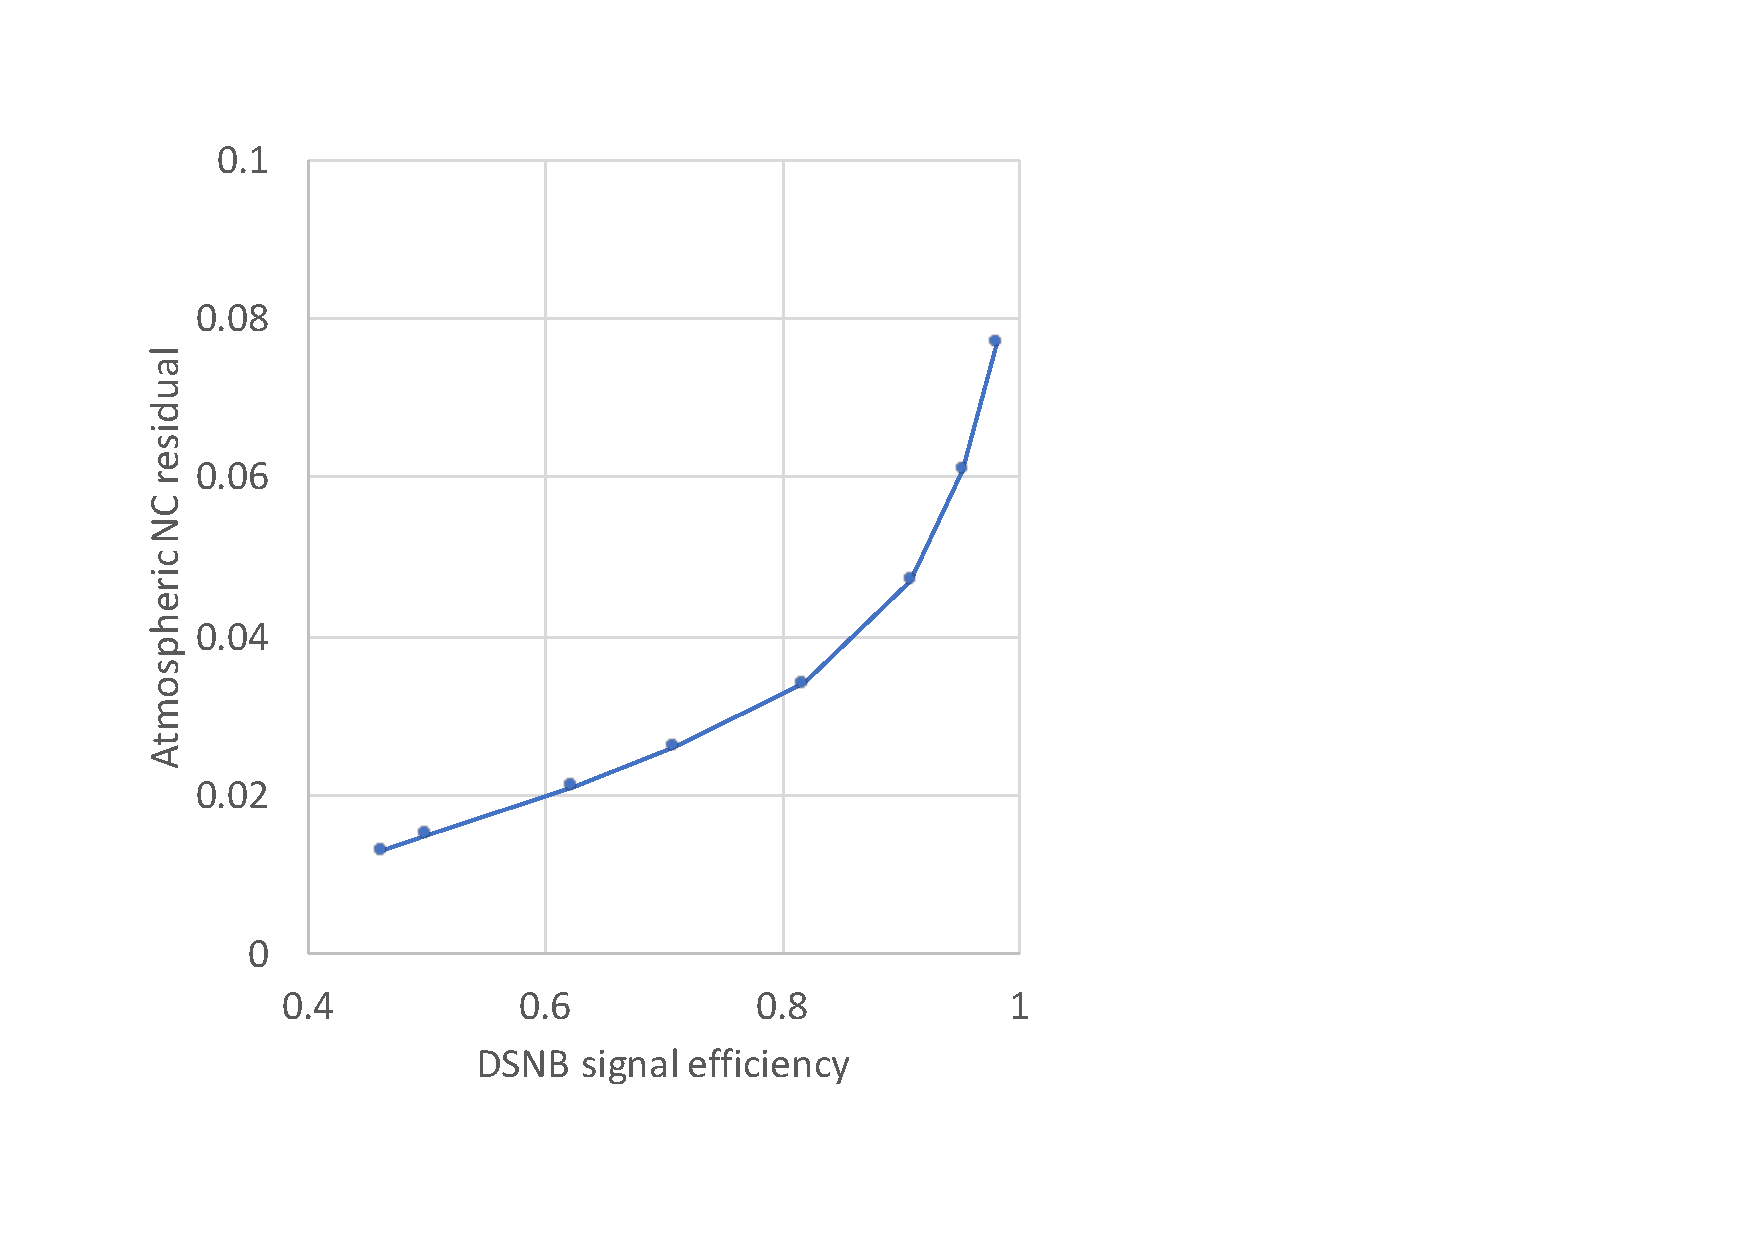
\includegraphics[width=0.39\textwidth]{pics/dsnb_cs_efficiencies}
\caption{{\it Left panel:} The Cherenkov-to-scintillation (C/S) ratio offers a powerful tool for the discrimination of positron-like DSNB ({\it blue}) and hadronic prompt events from atm-NC reactions ({\it red}) that feature low Cherenkov emission. While the majority of background events features a C/S ratio of 0, final-state $\gamma$-rays results in a curved band of atm-NC events leaking into the signal region ({\it inset panel}). These can be effectively discriminated by cutting on the C/S ratio: the {\it right panel:} shows the residual fraction of atm-NC as function of the remaining signal efficiency for DSNB events.}
\label{fig:dsnb_csratio}
\end{figure}

\subsubsection{Sensitivity to the DSNB signal} 

%Based on WbLS, THEIA offers excellent background discrimination capabilities complementary to those of pure Water Cherenkov or Organic Scintillator Detectors. 

\begin{table}[htp!]
\begin{center}
\begin{tabular}{lccccc}
\hline
Spectral contribution			& before cuts & Li veto & delayed decays & C/S cut & single-ring \\
\hline
DSNB signal				& 21.1	& 20.9	& 20.9	& 20.5	& 20.5\\
Reactor neutrinos			& $-$	& $-$ 	& $-$	& $-$	& $-$ \\
Atmospheric CC			& 2.1		& 2.1		& 2.1		& 2.0		& 2.0 \\
\hline
Atmospheric NC			& 436	& 432 	& 230	&11.5	& 6.2 \\
$\beta n$-emitters ($^9$Li)	& 55.1 	& $-$	& $-$	& $-$	& $-$ \\
fast neutrons				& 0.65 	& 0.65  	& 0.65	& $-$	& $-$ \\
\hline
Signal-to-background		& 0.043	& 0.048	& 0.090	& 1.52 	& 2.50  \\
\hline
\end{tabular}

\end{center}
\caption{Rates of DSNB signal and backgrounds within the observation window (8-30\,MeV) for a live exposure of 100\,kt$\cdot$years. While the first column represents the rates before cuts, the following columns apply delayed decay, C/S ratio and ring-counting cuts. The cited fast neutron rate assumes a 2.5\,m fiducial volume cut or presence of corresponding active shielding surrounding the target volume.}
\label{tab:dsnb_rates}
\end{table}

Tab.~\ref{tab:dsnb_rates} illustrates the impact of the aforementioned discrimination techniques on the signal and background rates within the observation window. While all background components including the atm-NC events are greatly reduced, the DSNB signal acceptance is hardly affected. THEIA at 50 kt will collect more signal events per year than SK-Gd and JUNO combined, reaching about {\cal O}(100) events over 10 years of measuring. The corresponding energy spectra are shown in Fig.~\ref{fig:dsnb_spectrum}b), demonstrating a clear dominance of the signal especially over the entire energy window. Beyond a $5\sigma$ discovery of the signal, THEIA will thus allow a first spectroscopic analysis of the DSNB signal. What is more, the dual detection of Cherenkov and scintillation signals will allow a in-depth study of the atm-NC events, supporting the systematic analyses of the corresponding backgrounds in JUNO and SK-Gd.

%\noindent A positive detection of the DSNB at a high significance level seems therefore well within reach even of a moderately sized (i.e.~20\,kt fiducial mass) detector. However, it is not immediately clear how much information can be extracted from a spectroscopic measurement on the red-shift dependent SN rate or the average SN neutrino spectrum. This depends not only on THEIA's properties alone but also on the event statistics and performance of SK-Gd and JUNO by the time of running.

%ADD here a text on the determination of the ratio of failed SNe

%\begin{figure}[htp!]
%\centering
%\includegraphics[width=0.75\textwidth]{dsnb/dsnb_after_cuts}
%\caption{The DSNB and background spectra expected following the application of all cuts lined out in tab.~\ref{tab:dsnb_rates}. While the signal rate is hardly reduced compared to fig.~\ref{fig:dsnb_spectrum}, it is now the dominant contribution in the spectrum.}
%\label{fig:dsnb_spectrum_after_cuts}
%\end{figure}

%\paragraph{Detector Requirements}
%As lined out above, the combination of Cherenkov and scintillation photons is a very powerful handle for background discrimination in THEIA. Moreover, it is a piece of complementary information that will not be available in pure water(+Gd) or organic LS detectors, giving the WbLS concept a real edge when addressing detection systematics. Optimum C/S determination power will be obtained when Cherenkov and scintillation light emission are at a similar intensity level. Therefore. an admixture of the organic phase of order 10\,\% to the WbLS will be most favorable for purposes of the DSNB.

%Moreover, a $5\sigma$-discovery of the DSNB, and even more so, a first attempt at its spectroscopy will crucially depend on the available statistics. Therefore, it is important to realize a large detector on the scale of 50\,kt target mass or beyond in order to make maximum use of the excellent WbLS detection capabilities.
